\chapter[Introdução]{Introdução} \label{cap:introducao}

A democracia digital é resumida por \citeonline{penteadoencontro} como o uso da Internet para consolidação da democracia.
\citeonline{marques2008participaccao}, com base em seu levantamento de outros estudos na temática, afirma que este uso
eleva a aplicação das atividades democráticas em diversos aspectos, principalmente, em relação a agilidade e quantidade
de informações transferidas de uma pessoa para outra. \citeonline{mendoncca2011democracia} também relatam a importância da tecnologia
para aproximação dos cidadãos e da política, através de novas formas de participação. 

Por essa razão, interessados passaram a analisar esse fenômeno, notando um crescente número de discussões acerca de temas políticos 
e uma polarização das mensagens trocadas,
principalmente em redes sociais. \citeonline{empurrandojuntos} afirmaram que as discussões realizadas
acabavam refletindo sempre o ponto de vista da maioria, resultando em pessoas sempre presentes em uma bolha de opinião. \citeonline{marques2008participaccao}
apresenta este ponto como um dos malefícios dessa nova forma de participação política, ao relatar sobre a influência de grandes grupos 
sobre os assuntos apresentados.

Além da relação de evidência de opiniões desses grupos dominantes, os algoritmos
das plataformas comumente utilizadas, em sua maioria, selecionam o conteúdo a ser apresentado de acordo com o comportamento anterior,
no qual foi coletada a opinião deste usuário. Essas características reforçam a formação das bolhas de opinião, 
dificultam a explanação das ideias da minoria e restringem a apresentação de pensamentos diferentes para quem usa essas plataformas. 

Nesse sentido, surge uma nova geração de plataformas sociais com o intuito de tornar essas discussões mais efetivas 
e evidenciar todas as opiniões, inclusive a da minoria. O Instituto Cidade Democrática\footnote{Site do Cidade Democrática: \url{http://www.cidadedemocratica.org.br/}},
tem trabalhado em uma ideia para esse tipo de plataforma. Entitulado de ``Empurrando Juntos'', 
trata-se de um software livre que tem como requisito principal agrupar pessoas que votaram de forma parecida, 
possibilitando uma fácil visualização das semelhanças e divergências nas opiniões acerca de um assunto \cite{empurrandojuntos}. 

A ideia é que um usuário entre em um \textit{website} ou em um aplicativo de celular para criar e participar de conversas, 
por meio da criação de comentários e atribuição de ``votos'' em comentários de outros usuários.
Os votos são realizados para concordar ou discordar do comentário realizado, semelhante ao conceito de \textit{like} ou \textit{dislike}.
A partir desta interação o sistema é responsável por formar os grupos de pessoas, em tempo real, de acordo com a semelhança nas opiniões.

Na ausência de um estabelecimento prévio dos conjuntos de pessoas, técnicas de classificação podem ser utilizadas para os agrupamentos
levando em consideração os dados em comum entre os usuários, que são os votos nos comentários.
De acordo com \citeonline{tan2013data, han2011data, clustering_review}, essas técnicas
têm como objetivo encontrar um modelo que possa descrever e distinguir classes de dados.
Sendo assim, nota-se a necessidade de um processo de classificação para que esses grupos sejam formados.

É possível dividir então o sistema em dois processamentos: 
gestão de usuários e conversas e agrupamento de pessoas com opinião semelhante. 
Observando isto em conjunto com a possibilidade do uso de diferentes técnicas para classificação 
e a característica do ``Empurrando Juntos'' de ser uma aplicação multiplataforma, notou-se
a necessidade do estabelecimento de uma arquitetura modularizada e do provimento dos serviços necessários para a realização
dos dois processamentos.

Segundo \citeonline{wagh2012comparative, understanding_web}, uma \textit{Application Programming Interface} (API)
é uma interface que expõe os seus componentes como um serviço, permitindo que outras aplicações interajam com esses 
componentes. Desse modo, possibilita o compartilhamento dos dados armazenados com as aplicações que a consomem.

Portanto, o objetivo do trabalho foi implementar uma API que sirva como contribuição para o ``Empurrando Juntos'',
capaz de fornecer os serviços de gerenciamento das conversas e de agrupamento de usuários, de forma que seja possível substituir
o método de classificação utilizado para o agrupamento.

Para realização do objetivo proposto, o trabalho foi dividido em cinco etapas, conforme a Figura \ref{fig:etapas_trabalho}. 

\begin{figure}[h!]
\centering
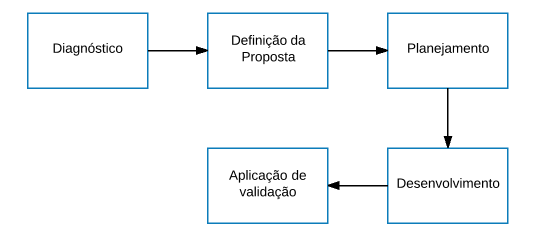
\includegraphics[scale=0.6]{figuras/etapas.png}
\caption{Etapas do trabalho}
\label{fig:etapas_trabalho}
\end{figure}

A etapa de ``Diagnóstico'' compreendeu o entendimento do escopo da plataforma ``Empurrando Juntos''. 
A etapa de ``Definição da Proposta'' foi caracterizada pela definição de escopo, 
da arquitetura da API e da comunicação com os módulos matemáticos. Na terceira etapa, 
foi feito o planejamento da execução do trabalho com o estabelecimento
de um cronograma das atividades das próximas etapas. 

Na etapa de ``Desenvolvimento'' foram realizadas as iterações de implementação, teste e adaptação da API. 
Por fim, na etapa de ``Aplicação de validação'', a título de validação da arquitetura proposta,
a API foi utilizada em um cenário de exemplo em comunicação com os outros dois módulos: cliente e matemático.

Nesse contexto, este trabalho, além desta introdução, está organizado em outros seis capítulos.
No Capítulo \ref{cap:empurrandojuntos} é apresentada a descrição, histórico e o escopo da plataforma ``Empurrando Juntos''.
O Capítulo \ref{cap:classificação} aborda os conceitos de classificação, com foco em uma das técnicas implementadas na plataforma. 
A definição da proposta e o planejamento são apresentados no Capítulo \ref{cap:proposta}.
A API desenvolvida no trabalho é apresentada no Capítulo \ref{cap:api}. No Capítulo \ref{cap:aplicacao_exemplo} é
apresentada uma validação da API. E por fim são apresentadas as conclusões no Capítulo \ref{cap:consideracoes_finais}.
